\begin{figure}
\pgfplotsset{width=\textwidth}
\centering
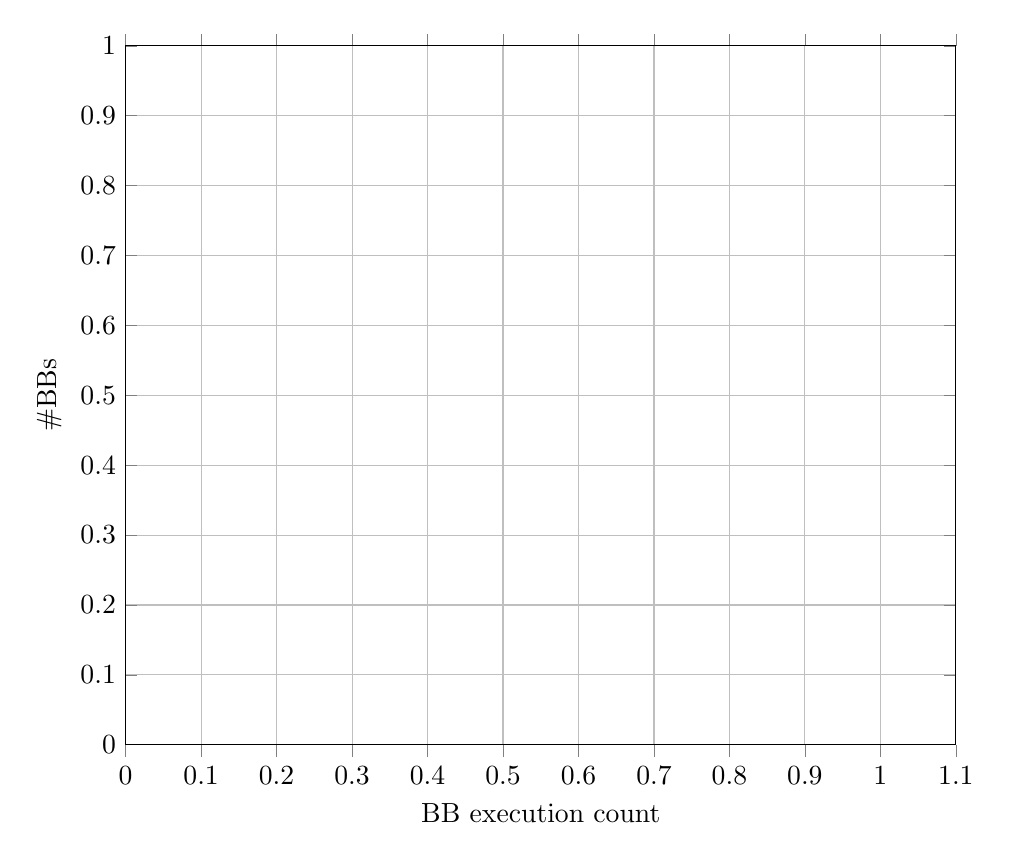
\begin{tikzpicture}
\begin{axis}[
	ybar,
	xlabel={BB execution count},
	ylabel={\#BBs},
	xmin=0,
	ymin=0,
	ymax=20,
	grid=both,
	%bar width=0.5cm,
]

\runtex{counter-dist1 -g dota}

\node at (axis cs:15e9,19) {\color{white}↑};
\end{axis}
\end{tikzpicture}
\captionof{figure}{The distribution of counter values on basic blocks of Dota 2}
\label{dia:counter_values}
\end{figure}
